\documentclass[beamer]{standalone}

\usetheme{naked}
\setbeamercolor{alerted text}{fg=green!50!black}
\setbeamercolor{box title}{fg=purple}
\setbeamertemplate{frametitle}{}

% \usepackage{xkeyval}
% \usepackage{pgffor}

\usepackage{standalone}

\makeatletter
../code-graphs.tex
\makeatother

% vertical centering of cells
% see http://tex.stackexchange.com/questions/46386/vertically-center-cells-of-a-table
\usepackage{array}% http://ctan.org/pkg/array
\newcolumntype{M}{>{\centering\arraybackslash}m{\dimexpr.17\linewidth-2\tabcolsep}}

% remove space between margin and lists
\usepackage{enumitem}
\setitemize{label=\usebeamerfont*{itemize item}%
  \usebeamercolor[fg]{itemize item}
  \usebeamertemplate{itemize item}}
\setlist{leftmargin=*,labelindent=0cm}

%\usepackage{amsmath}

\usepackage{tikz}
\usepackage{tkz-graph}
\usepackage{tkz-berge}
\usepackage{tkz-berge-add}

\usepackage[utf8]{inputenc}
% \usepackage{libertine}
% \usepackage[libertine]{newtxmath}

%\usepackage{lxfonts}

\usepackage{cabin}
\usepackage{mathastext}

\newcommand{\graphcaption}[4][gray!80!white]{\draw (#2,#3) node [fill=#1]{#4};}

\SetVertexSimple[FillColor=gray, MinSize=10pt, LineWidth=1.5pt]

\tikzset{EdgeStyle/.style= {%
    color           = white,
    double          = black,
    double distance = 2.5pt}}

\newcommand{\setof}[2]{\left\{\,#1\mid #2\,\right\}}

\newcommand{\triangulo}[4]{%
  \shadedraw[inner color=#4,opacity=0.8,line width=1pt]
  (#1.center) -- (#2.center) -- (#3.center) -- cycle;}

\newcommand{\triangleshaded}[3]{%
  \draw[fill=gray]
  (#1.center) -- (#2.center) -- (#3.center) -- cycle;}

\newcommand{\triang}[3]{%
  \shadedraw[inner color=gray,,opacity=0.8,line width=1pt]
  (#1.center) -- (#2.center) -- (#3.center) -- cycle;}

\begin{document}

\begin{standaloneframe}

  \vspace{\fill}
  
  \uncover<1->{%
    \begin{minipage}{0.6\linewidth}
      Una colección $\mathcal{C}$ de subconjuntos de $X$ es
      \alert{intersecante} si $Q_{1},Q_{2}\in\mathcal{C}$ implica
      $Q_{1}\cap Q_{2}\ne\emptyset$.
    \end{minipage}}%
  \uncover<2->{%
    \begin{minipage}{0.4\linewidth}
      \centering
      \scriptsize
      $\mathcal{C}=\{\{1,2\},\{1,3\},\{2,3\}\}$
    \end{minipage}}

  \vspace{\fill}

  \uncover<3->{%
    \begin{minipage}{0.6\linewidth}
      Una gráfica $G$ es \alert{Helly} si cualquier colección
      $\mathcal{C}$ intersecante de clanes es tal que
      $\cap\mathcal{C}\ne\emptyset$. 
    \end{minipage}}%
  \uncover<4->{%
    \begin{minipage}{0.4\linewidth}
      \centering
        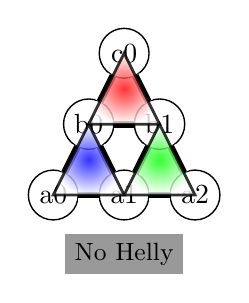
\begin{tikzpicture}[scale=0.5]
          \grPath[RA=1.8,prefix=a,form=2]{3}
          \grPath[RA=1.8,prefix=b,form=2,y=1.8]{2}
          \grPath[RA=1.8,prefix=c,form=2,y=3.6]{1}

          \Edges(a0,b0,c0,b1,a2)
          \Edges(b0,a1,b1)

          \only<5>{%
            \triangulo{a0}{a1}{b0}{blue}
            \triangulo{a2}{a1}{b1}{green}
            \triangulo{b0}{b1}{c0}{red}}
          \uncover<6->{\graphcaption{0}{-1.5}{\small No Helly}}
        \end{tikzpicture}
    \end{minipage}}

  \vspace{\fill}

\end{standaloneframe}

\end{document}
